\documentclass[11pt]{article}
\usepackage{nodalida2017}
\usepackage{mathptmx}
\usepackage{xcolor}
\usepackage{graphicx}
\usepackage{url}
\usepackage{latexsym}
\usepackage{fancyvrb}
\special{papersize=210mm,297mm} 


\title{Exploring the Expressivity of Constraint Grammar}

\author{%
  Pepijn Kokke \\
  University of Edinburgh \\
  {\tt pepijn.kokke@ed.ac.uk} \\\And
  Inari Listenmaa \\
  University of Gothenburg \\
  {\tt inari.listenmaa@cse.gu.se} }

\date{\today}

\def\t#1{\texttt{#1}}
\def\h#1{{\tt \color{gray} #1}}
\def\swf{\h{"<s>"}}
\def\maxAmb#1{$\langle \Sigma \rangle_#1$}
\def\maxAmbFSA#1{$\langle \Sigma,S \rangle_#1$}
\def\maxAmbCFG#1{$\langle \Sigma,\Sigma^{\prime} \rangle_#1$}

\begin{document}
\maketitle

\begin{abstract}
  We believe that for any formalism which has its roots in linguistics, it is a
  natural question to ask ``how expressive is it?'' Therefore, in this paper, we
  begin to address the question of the expressivity of CG.
  Aside from the obvious theoretical interest, we envision also practical
  benefits. For instance, we hope that the FSA$\rightarrow$CG conversion tool, described in
  later sections of this paper, could eventually be developed to generate
  human-readable CG code from regular expressions or a context-free grammar. 
\end{abstract}


\section{Introduction}
For any formalism with its root in linguistics, it is natural to ask questions
such as ``How expressive is it?'' or ``Where does it sit in the Chomsky
hierarchy?''~\cite{chomsky1956hierarchy}
In this paper, we begin addressing some of these questions for constraint
grammar~\cite[CG]{karlsson1995constraint}.

Before we can even consider such a question, there is a problem we must
solve. CG was never meant to be a grammar in the generative sense. Instead, it
is a tool for analysing and disambiguating strings.
This, we believe, explains why the question of the expressivity of CG went
unasked and unanswered for a long time.
%WEN: How much would this upset Anssi? Has he actually looked into its
%     expressivity?
It also gives us our first problem: How do we view CGs generatively?
We address this in section~\ref{sec:gencg}.


\section{Generative Constraint Grammar}\label{sec:gencg}
We view a constraint grammar CG as generating a formal language $\mathcal{L}$
over an alphabet $\Sigma$ as follows.
We encode words $w \in \Sigma^\star$ as a sequence of cohorts, each of which has
one of the symbols of $w$ as a reading.
A constraint grammar CG rejects a word if, when we pass its encoding through the
CG, we get back the cohort \t{"<REJECT>"}. A constraint grammar CG accepts a word
if it does not reject it.
We generate the language $\mathcal{L}$ by passing every $w \in \Sigma^\star$
through the CG, and keeping those which are accepted.

As an example, consider the language $a^\star$ over $\Sigma = \{a,b\}$.
This language is encoded by the following constraint grammar:
\begin{center}
  \begin{Verbatim}
    LIST A = "a";
    LIST B = "b";
    SET LETTER = A OR B;
    SELECT A;
    ADDCOHORT ("<REJECT>")
        BEFORE LETTER 
        IF (-1 (>>>) LINK 1* B);
    REMCOHORT LETTER
        IF (-1* ("<REJECT>"));
  \end{Verbatim}
\end{center}
We then encode the input words as a series of letter cohorts with readings
(e.g.\ \(\t{"<l>"}\;\t{"a"}\), \(\t{"<l>"}\;\t{"b"}\)), and run the grammar.
For instance, if we wished to know whether either word in $\{aaa,aab\}$ is part
of the language $a^\star$, we would run the following queries:
\begin{center}
  \begin{tabular}{l|c}
    \textbf{Input}         & \textbf{Output} \\ \hline
    \(\t{"<l>"}\;\t{"a"}\) & \(\t{"<l>"}\;\t{"a"}\) \\
    \(\t{"<l>"}\;\t{"a"}\) & \(\t{"<l>"}\;\t{"a"}\) \\
    \(\t{"<l>"}\;\t{"a"}\) & \(\t{"<l>"}\;\t{"a"}\) \\ \hline
    \(\t{"<l>"}\;\t{"a"}\) & \t{"<REJECT>"} \\
    \(\t{"<l>"}\;\t{"a"}\) \\
    \(\t{"<l>"}\;\t{"b"}\)
  \end{tabular}
\end{center}
As CG is a tool meant for disambiguation, we can leverage its power to run both
queries at once:
\begin{center}
  \begin{tabular}{l|c}
    \textbf{Input}                  & \textbf{Output} \\ \hline
    \(\t{"<l>"}\;\t{"a"}\)          & \(\t{"<l>"}\;\t{"a"}\) \\
    \(\t{"<l>"}\;\t{"a"}\)          & \(\t{"<l>"}\;\t{"a"}\) \\
    \(\t{"<l>"}\;\t{"a"}\;\t{"b"}\) & \(\t{"<l>"}\;\t{"a"}\)
  \end{tabular}
\end{center}
This is a powerful feature, because it allows us disambiguate based on some
formal language $\mathcal{L}$ if we can find the CG which generates it.
However, the limitations of this style become apparent when we look at a run of
a CG for the language $\{ab,ba\}$:
\begin{center}
  \begin{tabular}{l|c}
    \textbf{Input}                  & \textbf{Output} \\ \hline
    \(\t{"<l>"}\;\t{"a"}\;\t{"b"}\) & \(\t{"<l>"}\;\t{"a"}\;\t{"b"}\) \\
    \(\t{"<l>"}\;\t{"a"}\;\t{"b"}\) & \(\t{"<l>"}\;\t{"a"}\;\t{"b"}\) \\
  \end{tabular}
\end{center}
While the output contains the interpretations $ab$ and $ba$, it also includes
$aa$ and $bb$. Therefore, while this style is useful for disambiguating using
CGs based on formal languages, it is too limited to be used in defining the
language which a CG generates.
%WEN: we should include a reference to the other formalism here, or to the
%     discussion section in which we talk about the disjunction problem

In light of the idea of using CGs based on formal languages for disambiguating,
it seems at odds with the philosophy of CG to reject by replacing the entire
input with a single \t{"<REJECT>"} cohort. CG generally refuses to remove the
last possible reading of a cohort, under the philosophy that \emph{some}
information is certainly better than none.
However, for the definition of CG as a formal language, we need some sort of
distinctive output for rejections. Hence, we arrive at \emph{two} distinct ways
to run generative CGs: the method in which we input unambiguous strings, and
output \t{"<REJECT>"}, which is used in the definition of CG as a formal
language; and the method in which we input ambiguous strings, and simply
disambiguate as far as possible. 


\section{A lower bound for CG}
% WEN: We should move this section over into section 2 about GCG
It should be noted that VISL CG-3 \cite{bick2015,vislcg3} supports commands 
such as \t{EXTERNAL}, which runs an external executable. It should therefore 
be obvious that the complete set of CG-3 commands, at least theoretically, 
can generate any recursively enumerable language. For this reason, we restrict 
ourselves to a subset of the commands permitted by CG.

In this section, we will only use the \t{REMOVE} command with sections, in
addition to a single use of the \t{ADDCOHORT} command to add the special cohort
\t{"<REJECT>"}, and a single use of the \t{REMCOHORT} command to clean up
afterwards. 
We show that, using only these commands, CG is capable of generating some
context-free and context-sensitive languages, which establishes a lower bound on 
the expressivity of CG (see Figure~\ref{fig:nocorr}).
%
\begin{figure}[h]
  \centering
  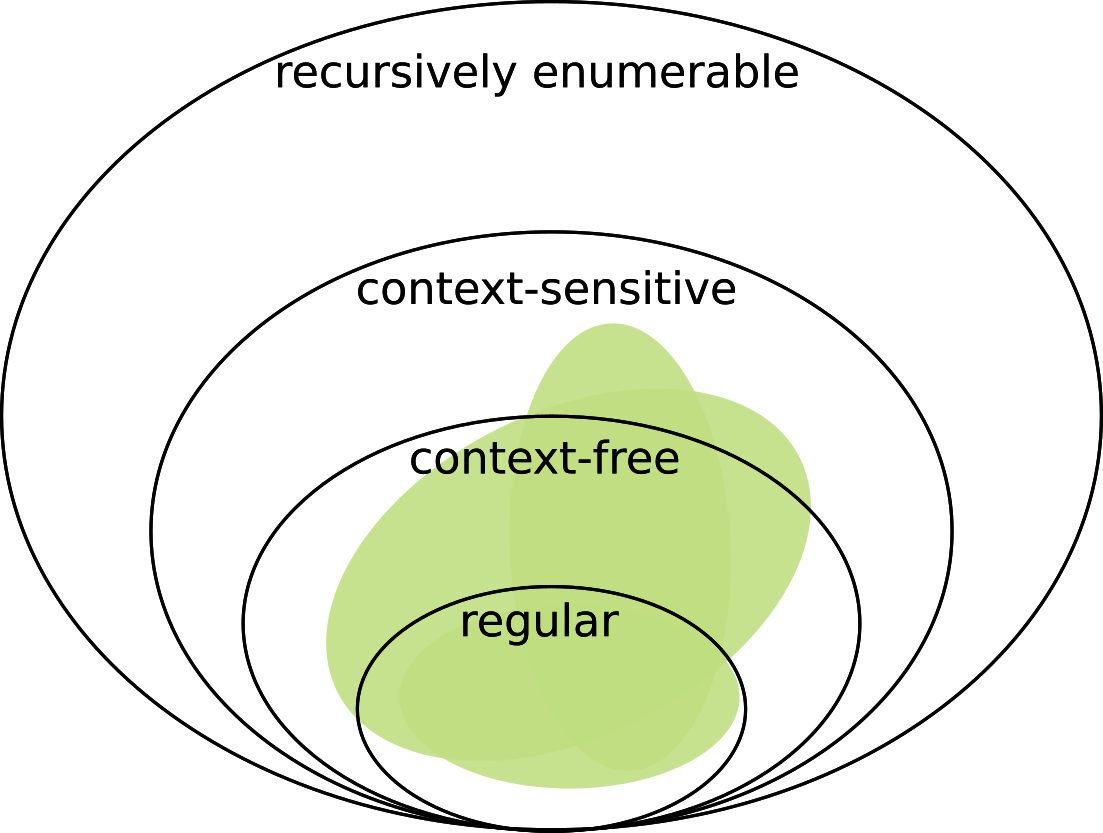
\includegraphics[width=0.8\linewidth]{chomsky}
  \caption{Lower bound on the expressivity of CG.}
  \label{fig:nocorr}
\end{figure}


\subsection{Example grammar: $a^nb^n$}
Below, we briefly describe the CG which generates the language $a^nb^n$.
This CG is defined over the alphabet $\Sigma$, in addition to a hidden alphabet
$\Sigma^\prime$. These hidden symbols are meant to serve as a simple form of
memory. When we encode our input words, we tag each cohort with \emph{every}
symbol in the hidden alphabet\footnote{
  We can automatically add these hidden symbols to our cohorts using a single
  application of the \t{ADD} command.
}, e.g.\ for some symbol $\ell \in \Sigma$ and $\Sigma' = \{h_1,\dots,h_n\}$ we
would create the cohort \(\t{"<\(\ell\)>"}\;\t{"h\(_1\)"}\;\dots\;\t{"h\(_n\)"}\).

% Pepijn's original:
%\(\t{"<l>"}\;\t{"\(\ell\)"}\;\t{"h\(_1\)"}\;\dots\;\t{"h\(_n\)"}\). 

% \begin{itemize}
% \item[] \t{"<\(\ell\)>"}
%  \begin{itemize}
%     \item[] \t{"h\(_1\)"} \\
%             \dots \\
%             \t{"h\(_n\)"}
%  \end{itemize} 
% \end{itemize}

The CG for $a^nb^n$ uses the hidden alphabet \{\t{odd}, \t{even}, \t{opt\_a},
\t{opt\_b}\}. These symbols mean that the cohort they are attached to is in an
even or odd position, and that $a$ or $b$ is a legal option for this cohort,
respectively. The CG operates as follows: 
\begin{enumerate}
\item
  Is the number of characters even? We know the first cohort is odd, and the
  rest is handled with rules of the form \t{REMOVE even IF (NOT -1 odd)}. If the
  last cohort is odd, then discard the sentence. Otherwise continue\dots
\item
  The first cohort is certainly $a$ and last is certainly $b$, so we can
  disambiguate the edges: 
  \t{REMOVE opt\_b IF (NOT -1 (*))}, and \t{REMOVE opt\_a IF (NOT 1 (*))}. 
\item
  Disambiguate the second cohort as $a$ and second-to-last as $b$, the third as
  $a$ and third-to-last as $b$, etc, until the two ends meet in the middle. If
  every \t{"<a>"} is marked with \t{opt\_a}, and every \t{"<b>"} with
  \t{opt\_b}, we accept. Otherwise, we reject.  
\end{enumerate}
The language $a^nb^n$ is context-free, and therefore CG must at least partly
overlap with the context-free languages.


\subsection{Example grammar: $a^nb^nc^n$}
We can extend the approach used in the previous grammar to write a grammar which
accepts $a^nb^nc^n$. Essentially, we can adapt the above grammar to find the
middle of any input string. Once we have the middle, we can ``grow'' $a$s from
the top and $b$s up from the middle, and $b$s down from the middle and $c$s up
from the bottom, until we divide the input into three even chunks.
If this ends with all \t{"<a>"}s marked with \t{opt\_a}, all \t{"<b>"}s marked
with \t{opt\_b}, and all \t{"<c>"}s marked with \t{opt\_c}, we accept.
Otherwise, we reject.

The language $a^nb^nc^n$ is context-sensitive, and therefore CG must at least
partly overlap with the context-sensitive languages. 


\begin{figure}[t]
  \centering
  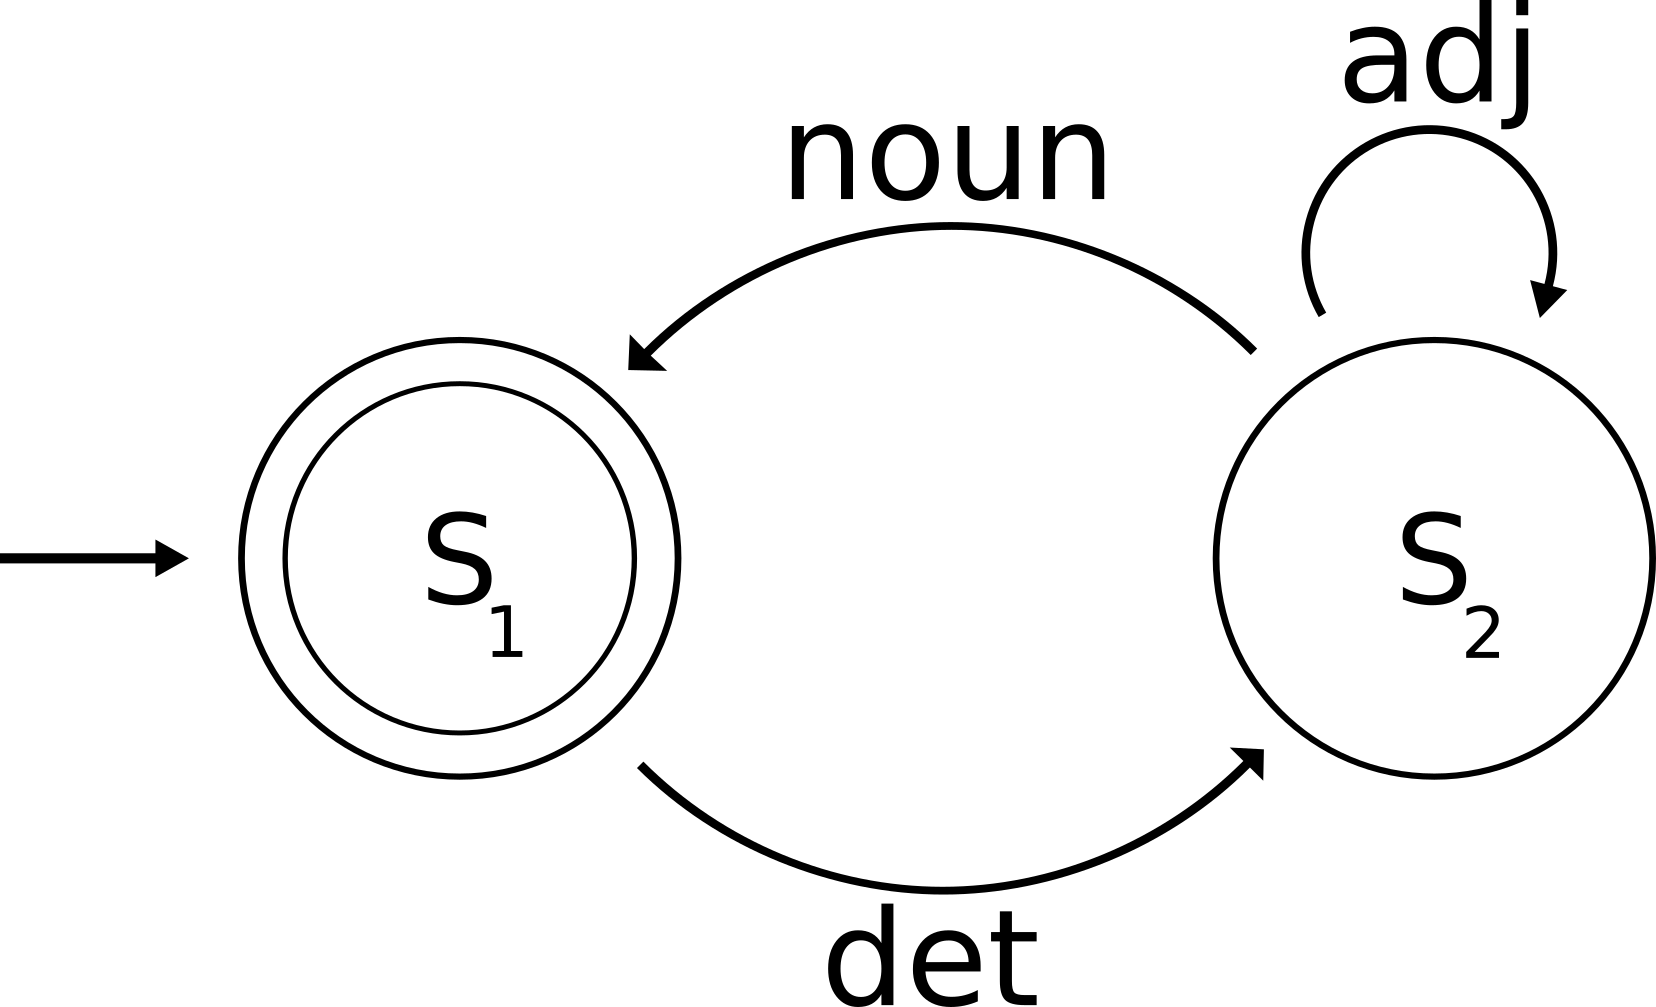
\includegraphics[width=0.6\linewidth]{fsa.png}
  \caption{A finite-state automaton describing the regular language \t{det
      (adj)* n}.}
 \label{fig:fsa}
\end{figure}


\section{Are all regular languages in CG?}
In the present section, we propose a method to transform arbitrary finite-state
automata into CG. Figure~\ref{fig:fsa} presents an example automaton with
$\Sigma = \{$\emph{det, adj, n}$\}$, for which we implement a corresponding CG
as follows.

\subsection{Cohorts and sentences}
As previously, we define a hidden alphabet $\Sigma^{\prime} = \{$\t{opt\_det,
  opt\_adj, opt\_n}$\}$, and insert the full set $\Sigma^{\prime}$ to each
cohort as readings. In addition, we introduce \emph{state cohorts}, which
contain the full set $S = \{s_1, s_2\}$. For example, the sequence \emph{det n}
would be modelled with the following sentence:
%
\begin{table}[h]
  \centering\small
  \begin{tabular}{c|c|c|c|c}
    \swf   & \t{"<det>"}  & \swf   & \t{"<n>"} & \swf   \\ \hline
    \h{s1} & \t{opt\_det} & \h{s1} & \t{opt\_det} & \h{s1} \\
    \h{s2} & \t{opt\_adj} & \h{s2} & \t{opt\_adj} & \h{s2} \\
           & \t{opt\_n}   &        & \t{opt\_n}   &        \\
     
  \end{tabular}
\end{table}

%
The rules of the grammar disambiguate both word cohorts and state cohorts. Thus
the desired result shows both the accepted string and the path in the automaton.

\begin{table}[h]
  \centering\small
  \begin{tabular}{c|c|c|c|c}
    \swf   & \t{"<det>"}  & \swf   & \t{"<n>"} & \swf   \\ \hline
    \h{s1} & \t{opt\_det}      & \h{s2} & \t{opt\_n}        & \h{s1} \\

  \end{tabular}
\end{table}



\subsection{Rules}
Given that every transition happens between two states, and every state 
has an incoming and outgoing transition, every rule needs only
positions -1 and 1 in its contextual tests. 
The semantics of the rules are ``remove an \t{opt\_POS} tag, if it is 
\emph{not} surrounded by allowed states'',
and ``remove a state, if it is \emph{not} surrounded by allowed transitions''.
For the example automaton, the \t{opt\_POS}-rules are as follows.
\begin{verbatim}
REMOVE...
  opt_det IF (NEGATE -1 S1 LINK 2 S2) ;
  opt_adj IF (NEGATE -1 S2 LINK 2 S2) ;
  opt_n   IF (NEGATE -1 S2 LINK 2 S1) ;
\end{verbatim}
\noindent The start and end states naturally correspond to the first and last
state cohort, and can be trivially disambiguated, in this case both into \t{s1}.
Once we remove a reading from either side of a cohort, some more rules can take
action---the context ``\t{s2} on the left side and \t{s1} on the right side''
may be broken by removing either \t{s2} or \t{s1}. 

If there is only one allowed string of length $n$ in the language, then the
result should have only one \t{opt\_POS} reading per cohort, and we proceed to
check whether they correspond to the original word forms \t{"<POS>"}: if
\t{opt\_det} is the only reading, the word form must be \t{"<det>"}, and so on.

If there are multiple strings of the same length in the language, we have to
relax our criteria: if every cohort with a reading \t{POS} has a corresponding
\t{opt\_POS} in the set of remaining readings, such as \{\t{det}, \t{opt\_det},
\t{opt\_adj}\}, we accept the string.


\paragraph{Real text}
Alternatively, we can apply this scenario to real-life ambiguities, where the word cohorts
contain only some subset of all the readings. 
In the following table, we show the initial state of the phrase ``the book''.
The word forms are now actual words, and the \t{\h{opt\_}POS} only include the actual analyses of those words.


\begin{table}[h]
  \centering\small
  \begin{tabular}{c|c|c|c|c}
    \swf   & \t{"<the>"}  & \swf  & \t{"<book>"} & \swf   \\ \hline
    \h{s1} & \t{\h{opt\_}det}     & \h{s1} & \t{\h{opt\_}n} & \h{s1} \\
    \h{s2} &                      & \h{s2} & \t{\h{opt\_}v} & \h{s2} \\

  \end{tabular}
\end{table}

In this scenario, we would omit matching word forms to \t{\h{opt\_}POS} tags; 
instead, it just becomes an alternative way of disambiguation.


\subsection{Limitations}
As we point out in Section~\ref{sec:gencg}, CG is not suited for handling disjunction;
the same problem with the language $\{ab,ba\}$ would happen here:

\begin{table}[h]
  \centering\small
  \begin{tabular}{c|c|c|c|c}
    \swf    & \t{"<a>"}  & \swf    & \t{"<b>"}  & \swf    \\ \hline
    \h{...} & \t{opt\_a} & \h{...} & \t{opt\_a} & \h{...} \\ 
            & \t{opt\_b} &         & \t{opt\_b} &                   
  \end{tabular}
\end{table}

As \newcite{lager_nivre01} point out, CG has no way of expressing disjunction.
Unlike its close cousin FSIG \cite{koskenniemi90}, which would represent this
language faithfully, CG substitutes uncertainty on the sentence level (``either
$ab$ or $ba$'') with uncertainty in the cohorts: ``the first character may be
either $a$ or $b$, and the second character may be either $a$ or $b$''.
Given that this is a fundamental design of CG, we do not envision a way out of 
this limitation, except for the generating multiple CGs per automaton.

However, it is an unclear how much this property would limit us in creating 
\emph{useful} CG rules out of more expressive grammar formalisms.
Applying the rules to real-life ambiguous cohorts is expected to be easier:
those cohorts are not \maxAmb{n}, but some much smaller subset of $\Sigma$.
Hence, despite the theoretical limitation, we are still hopeful
for more applied use cases.


\section{Discussion}

At the time of writing, the grammars generated by the FSA$\rightarrow$CG
conversion tool look awkward, and involve a number of extra cohorts and symbols.
However, it does give us the ability to quickly generate fragments of CG code
which disambiguate or rewrite input based on a regular expression.
We are hoping to develop this further, to also include context-free or even
mildly context-sensitive grammars.
Such CGs could be used as, e.g.\ as part of a larger constraint grammar.
In addition, we would like to focus on making the grammars more human-readable,
so that they could be used to quickly generate a basis for a constraint grammar
from existing context-free grammars (or equivalent formalisms).
This could serve as an alternative to learning grammars from a corpus.


\section{Related Work}
\newcite{tapanainen1999phd} gives an account of the expressivity of
the contextual tests for 4 different constraint formalisms, including CG. 
In addition, parsing complexity can be easily defined for a given variant and 
implementation of CG; see for instance \newcite{nemeskey14}.
\cite{ylijyra2017} presents questions regarding the expressive power
of Constraint Grammar, but concentrates on the implementation side.
To our knowledge, CG as a generative model has not been been approached before.

\bibliographystyle{acl}
\bibliography{cg}

\end{document}
